% 角平分线核心性质：P 在平分线上 + PM⊥OA + PN⊥OB → PM = PN
\documentclass[tikz,border=4pt]{standalone}
\usepackage{ctex}
\usepackage{amsmath}
\usetikzlibrary{calc, decorations.markings, arrows.meta}
\begin{document}
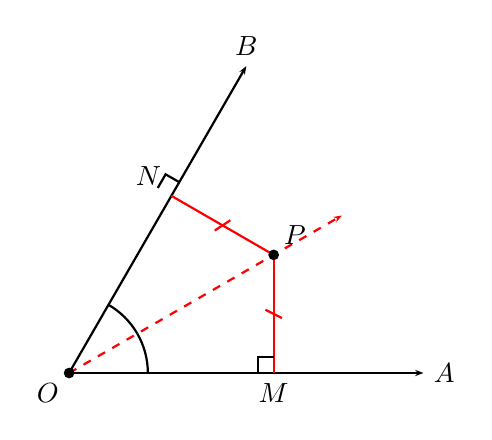
\begin{tikzpicture}[scale=1.0, thick,
  tick/.style={postaction={decorate, decoration={markings,
    mark=at position 0.5 with {\draw (-1.5pt,-3pt) -- (1.5pt,3pt);}}}}]
  \coordinate (O) at (0,0);
  \coordinate (A) at (4.5, 0);
  \coordinate (B) at ({4.5*cos(60)}, {4.5*sin(60)});
  \draw[-{Stealth[length=3pt]}] (O) -- (A);
  \draw[-{Stealth[length=3pt]}] (O) -- (B);
  % 角平分线方向 30°
  \draw[red, dashed, -{Stealth[length=3pt]}] (O) -- ({4.0*cos(30)}, {4.0*sin(30)});
  \coordinate (P) at ({3.0*cos(30)}, {3.0*sin(30)});
  \coordinate (M) at ({3.0*cos(30)}, 0);
  \pgfmathsetmacro{\proj}{3.0*cos(30)*cos(60)+3.0*sin(30)*sin(60)}
  \coordinate (N) at ({\proj*cos(60)}, {\proj*sin(60)});
  \draw[tick, red] (P) -- (M);
  \draw[tick, red] (P) -- (N);
  % 直角符号 at M
  \draw ($(M)+(-0.2,0)$) -- ($(M)+(-0.2,0.2)$) -- ($(M)+(0,0.2)$);
  % 直角符号 at N
  \draw ($(N)+({0.2*cos(150)}, {0.2*sin(150)})$)
     -- ($(N)+({0.2*cos(150)+0.2*cos(60)}, {0.2*sin(150)+0.2*sin(60)})$)
     -- ($(N)+({0.2*cos(60)}, {0.2*sin(60)})$);
  % 平分角弧
  \draw (1.0,0) arc (0:30:1.0);
  \draw ({1.0*cos(30)}, {1.0*sin(30)}) arc (30:60:1.0);
  \filldraw (O) circle (1.5pt);
  \filldraw (P) circle (1.5pt);
  \node[below left] at (O) {$O$};
  \node[right] at (A) {$A$};
  \node[above] at (B) {$B$};
  \node[above right] at (P) {$P$};
  \node[below] at (M) {$M$};
  \node[above left] at (N) {$N$};
\end{tikzpicture}
\end{document}
